\section{Teknologi} % (fold)
\label{sec:Teknologi}

I dette afsnit bliver forskellige eksisterende teknologier bearbejdet med henblik på at give et overblik. Hver teknologi vil blive introduceret kort, hvorefter styrker og svagheder vil blive præsenteret. Dette kan senere bruges, når en løsning skal designes. Der beskrives både teknologier som Vestre Baadelaug allerede benytter, samt andre systemer, andre sejlklubber benytter. 

\subsection{Betalingssystem} % (fold)
\label{sub:tek_betaling}

I Vestre Baadelaug benyttes et chip-system til at håndtere betalinger fra gæster \cite{int_hf}. Der findes en automat til betaling af pladsbilletter, samt et system til el, bad og toilet.

Billetsystemet giver mulighed for at optanke et kort, eller bestille en dagsbillet. Ved bestilling af dagsbillet, skal gæsten indtaske bådens længde og gæstens nationalitet. Efter en fuldført betaling med kreditkort, udskrives en dagsbillet der skal ligge synligt på båden. Systemet er leveret af det danske firma BEAS. Den specifikke model Vestre Baadelaug benytter er \enquote{Billetautomat TMI}. Se \cref{fig:vb_systemer}.

\begin{figure}[h]
  \centering
  \begin{minipage}{0.45\textwidth}
    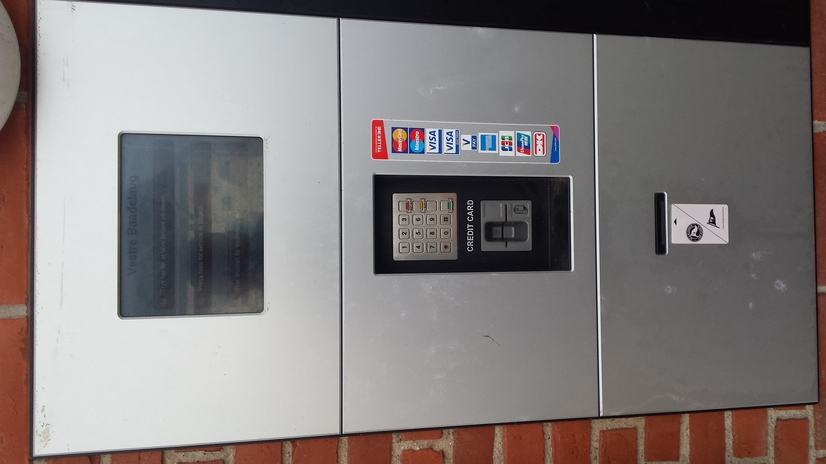
\includegraphics[angle=270,width=\textwidth]{vb_betalingssystem.jpg}
  \end{minipage}
  \begin{minipage}{0.45\textwidth}
    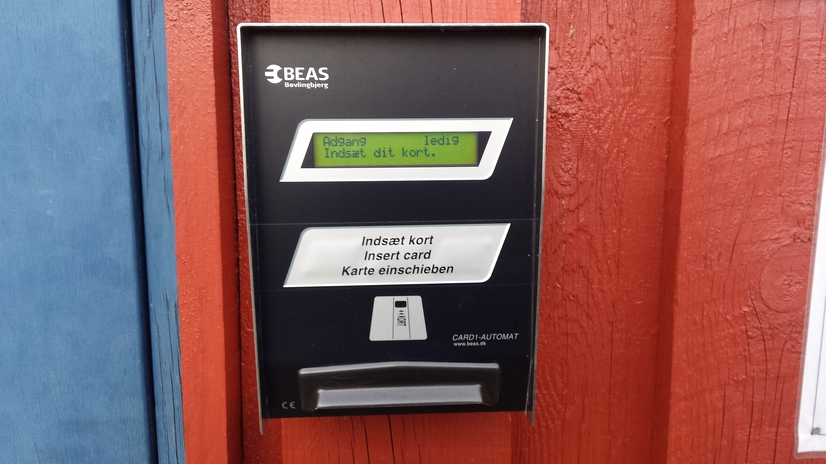
\includegraphics[width=\textwidth]{vb_kortsystem.jpg}
    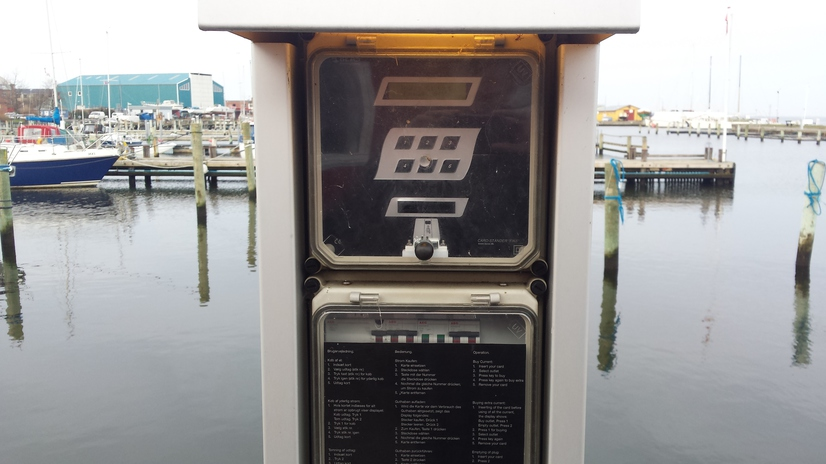
\includegraphics[width=\textwidth]{vb_elsystem.jpg}
  \end{minipage}
    \caption{Betalingssyste, kortsystem og elsystem set på Vestre Baadehavn}
    \label{fig:vb_systemer}
\end{figure}

Derudover benytter Vestre Baadelaug sig også af et chip-system til adgangskontrol til bad- og toiletfaciliteter, samt et system til el. Se \cref{fig:vb_systemer}.

\subsection{Håndtering af gæster - havnefogeden} % (fold)
\label{sub:gaster_havnefogeden}

Når havnefogeden skal holde styr på hvilke gæster der har betalt, benytter han sig af et bånd-system \cite{int_hf}. En mandag kan båndene være f.eks.\ røde, hvorefter de den næste dag kan være blå. På den måde kan havnefogen, når betalende både har synliggjort båndet på deres båd, se om gæsterne har betalt for dagen.

Et andet system havnefogeden bruger, er det der markererer hvorvidt gæster kan fortøje deres båd til en specifik plads. Det virker ved, at når et medlem sejler ud, bliver hans plads ledig, så derfor vender vedkommende et skilt foran pladsen. Dette skilt viser nu grønt, som tegn på at en gæst må holde på pladsen. Se \cref{fig:skilte}. Medlemmer kan meddele havnefogeden om hjemkomst, således at havnefogeden kan frigøre deres plads, inden de er i havnen. Dette sker via telefon eller forgående mundtlig aftale.

\begin{figure}[h]
  \centering
  \begin{minipage}{0.30\textwidth}
    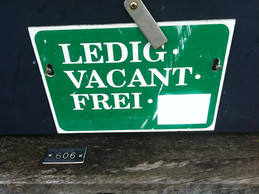
\includegraphics[width=\textwidth]{skilt_gron.jpg}
  \end{minipage}
  \begin{minipage}{0.30\textwidth}
    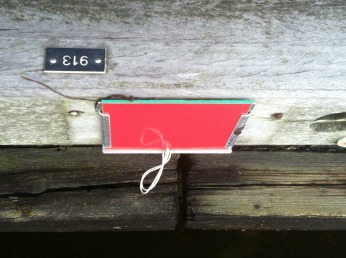
\includegraphics[width=\textwidth]{skilt_rod.jpg}
  \end{minipage}
  \begin{minipage}{0.30\textwidth}
    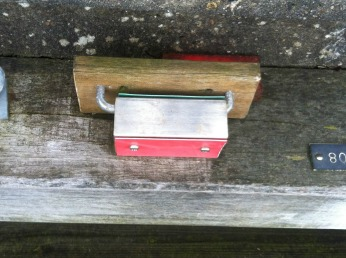
\includegraphics[width=\textwidth]{skilt_rod2.jpg}
  \end{minipage}
  \caption{Forskellige eksempler på skilte til markering af ledighed}
  \label{fig:skilte}
\end{figure}

\subsection{MarinaBooking.dk} % (fold)
\label{sub:MarinaBooking.dk}

Formålet med MarinaBooking \cite{marinabooking} er at gøre vandpladsreservationer lettere for gæster til lystbådehavne i Danmark. Systemet fungerer ved at gæster indtaster ankomst- samt afgangsdato, hvilken havn de vil lægge til og deres båds dimensioner. MarinaBooking kan med disse informationer nu præsentere et oversigtskort over havnebroerne på den specificerede havn, hvor gæsten kan vælge den ønskede vandplads på kortet. Systemet opkræver betaling, og gæsten har nu reserveret denne vandplads.

For at MarinaBooking kan fungere, skal lystbådehavne aktivt tilmelde sig. Dette kan de kun gøre, hvis de har en bro udelukkende dedikeret til gæster \cite{int_vb_sl}. I Vestre Baadelaug er dette som beskrevet i \cref{sec:gaste} ikke tilfældet.

MarinaBooking gør det enkelt for gæster fra Danmark, såvel som fra udlandet, at bestille havepladser fra internettet. Dette er godt for gæsterne, men også for administrationen i havnen, da tildeling af vandpladser herved ordner sig selv.

En af ulemperne ved MarinaBooking er det begrænsede udvalg af samarbejdshavne på hjemmesiden. Dette kan blandt andet skyldes ovenstående forklaring mht.\ gæstebroer.


%\subsection{E-conomic} % (fold)
%\label{sub:e-conomic}

%E-conomic er både navnet på en virksomhed og deres online regnskabsprogram. Formålet med programmet er at gøre økomnomi-håndtering let for selv ikke-regnskabsuddannede. E-conomic henvender sig primært til små- og mellemstore virksomheder \cite{economic}. Prisen for benyttelsen af E-conomic er abonnomentsbaseret med forskellige muligheder for tilpasninger. Da E-conomic kører online i en webbrowser, er alt data gemt og sikkerhedskopieret af E-conomic. Kunden ejer alt data med mulighed for eksportering efter abonnomentsophør.

%Fordelene ved e-conomic er den intuitive brugergrænseflade som letter mange bogførings handlinger. Derudover er programmet skrevet som et web-program hvilket gør at det kan tilgås fra alle platforme samt fra mange lokationer.

%\begin{figure}
%  \centering
%  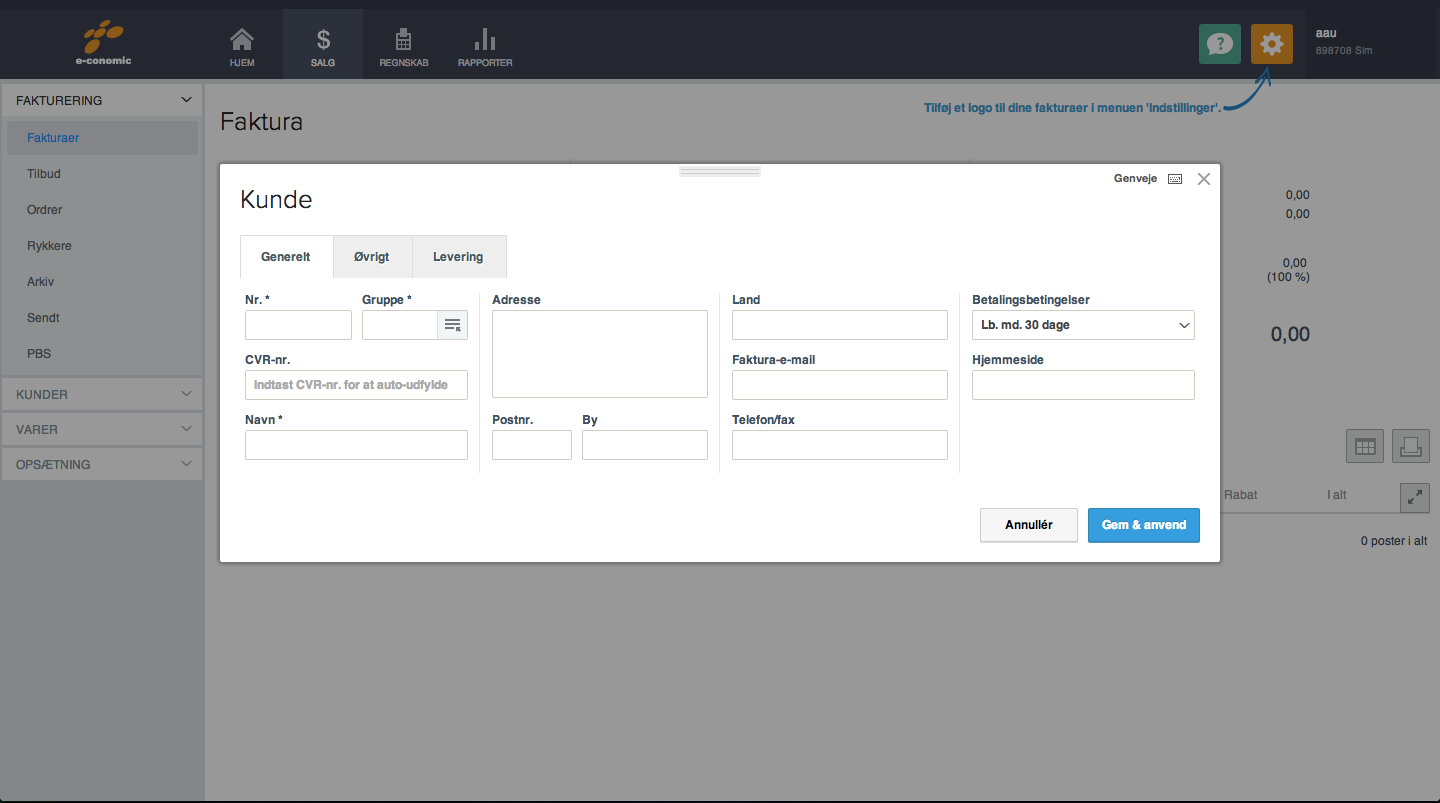
\includegraphics[width=\textwidth]{e-conomic.png}
%  \caption{Brugerinterface ved oprettelse af ny faktura - E-conomic}
%  \label{fig:e_conomic}
%\end{figure}


%Ulemperne ved e-conomic inkluderer afhængigheden af E-conomic med dertilhørende risiko for nedetid. 

\subsection{ForeningLet} % (fold)
\label{sub:ForeningLet}

ForeningLet er et online medlemssystem udviklet af Enteleki \cite{foreninglet}. Programmet har, som navnet antyder, specialiseret sig i systemer til foreninger. Det kan blandt andet håndtere medlemmer, regnskab, kontingent opkrævninger og bookning af materialer. Den årlige pris for programmet er afhængigt af antallet af medlemmer i foreningen, og desuden koster tillægsmoduler og dertilhørende ydelser ekstra. F.eks.\ koster et opkrævningsmodul 600 kr./år. Dertil kommer et tillæg på 80 øre per dannet opkrævning. I denne årlige pris er hosting, opdatering og vedligeholdelse inkluderet. ForeningLet holder altså styr på alle medlemsdata og gemmer dette på deres servere \cite{foreninglet}.

Navigationen i programmet foretages i en intuitiv brugerflade i en webbrowser. Man kan altså tilgå programmet på en hvilken som helst enhed med internetforbindelse. 

%\begin{figure}
%  \centering
%  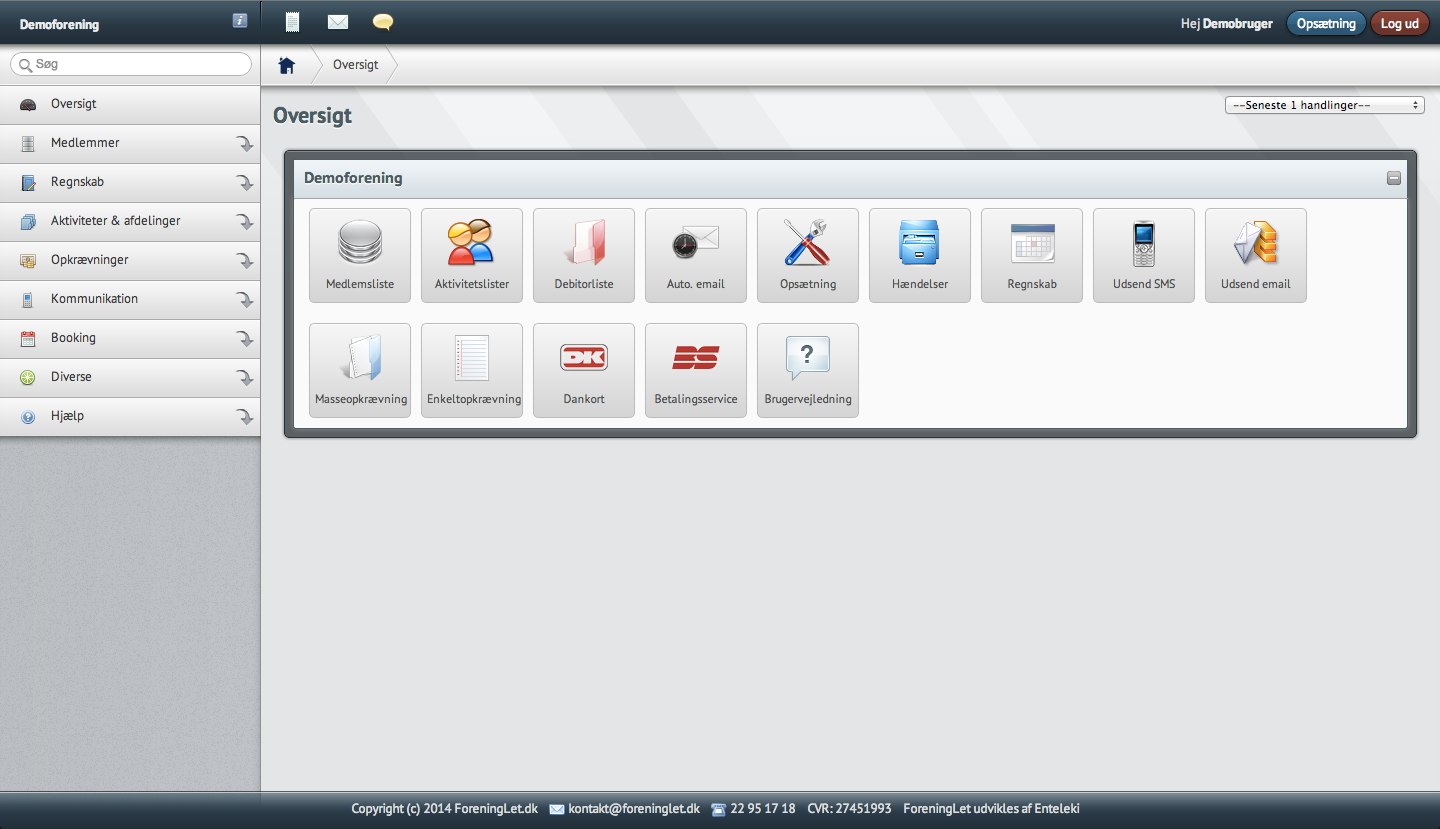
\includegraphics[width=\textwidth]{foreninglet.png}
%  \caption{Oversigt over brugergrænsefladen i ForeningLet}
%  \label{fig:foreninglet_program}
%\end{figure}

Selvom ForeningLet systemet er meget nemt at bruge, samt at sætte op, kan det blive omkostningsfuldt for foreninger med mange medlemmer. Dette skyldes førnævnte gebyrer på tillægsydelser som opkrævninger og rykkere. Derudover er foreningen afgængig af ForeningLet. Dette inkluderer både nedetiden for servicen og at datasikkerhedskopiering fungerer. Det vil altså sige at hvis ForeningLet en dag er nede, kan pågældende forening ikke benytte sig af systemet.
% subsection ForeningLet (end)

% section Teknologi (end)
